\documentclass{article}
\usepackage[utf8]{inputenc}
\usepackage{hyphenat}
\usepackage{enumitem}
\usepackage{framed}
\usepackage{graphicx}

% Coding packages
\usepackage{listings}
\usepackage{lmodern}
\usepackage{xcolor}
\usepackage{algorithm, algpseudocode}
\lstset{
  basicstyle=\ttfamily,
  literate={~} {\raise.17ex\hbox{$\scriptstyle\mathtt{\sim}$}}{1},
  columns=fullflexible,
  frame=single,
  breaklines=true,
  numbers=left,
  stepnumber=1,
  xleftmargin=2em,
  framexleftmargin=1.5em
}

\graphicspath{ {./images/} }

% Referencing
\usepackage[authordate,strict,backend=bibtex8,babel=other,bibencoding=inputenc]{biblatex-chicago}
\addbibresource{references}

% Create the Title 
\title{Finding New Pulsars Using Machine Learning}
\author{Jacob Ian Matthews \\ \\ Draft}

\begin{document}


% Build the title page
\begin{titlepage}
    
    \maketitle

    \section*{Abstract}

\end{titlepage}

\pagebreak

% Build Table of Contents
\tableofcontents

\pagebreak

% Start sections

% INTRODUCTION SECTION
\section{Introduction}

\subsection{Aim}

This project consists of three aims:
\begin{enumerate}[label=\roman*.]
    \item Investigate the use of Machine Learning (ML) techniques in surveying pulsars;
    \item Create a training dataset for a Machine Learning algorithm to find pulsars in data obtained by the Murchison Widefield Array (MWA); and
    \item Evaluate the utility of the Machine Learning algorithm used by the LOFAR Telescope for the Murchison Widefield Array, and adjust the algorithm as necessary to achieve optimum pulsar candidate generation.
\end{enumerate}

\subsection{Structure of this Report}

In this report, I will first explain in \emph{Section 1.3} how Pulsars, Radio Astronomy, and Machine learning work, and then explain what has been dubbed the ``Candidate Selection Problem" \autocite{lyon} and why Machine Learning is necessary in completing future pulsar surveys.

In \emph{Section 2} I discuss the methods undertook in: (i) developing the machine learning training dataset for the Murchison Widefield Array algorithm, and (ii) evaluating the machine learning algorithm used by the LOFAR surveys for use with the Murchison Widefield Array.

In \emph{Section 3} I analyse the results and findings obtained by the methods described in \emph{Section 2}, and in \emph{Section 4} I will discuss (i) the efficacy of the training datasets, and (ii) the usefulness of the LOFAR machine learning algorithm with the Murchison Widefield Array and why changes were made to the algorithm.

This report will end with my final conclusions on the use of machine learning in discovering new pulsars (\emph{Section 5}), and my recommendations to future researchers undertaking a similar project (\emph{Section 6}).

\subsection{Background Theory}

To answer the question of "what is a pulsar?" we must first investigate the evolution and death of stars.

A star can form when a cloud of hydrogen gas in the interstellar medium (ISM) collects mass over millions of years; as the mass of the gas cloud increases, its gravitational pull to gather more mass also increases \autocite{maoz}. This proto-star will eventually reach a critical mass in which the pressure of gravity within the gas causes enough friction between the gas particles to generate the required heat (thermal pressure) to begin fusing the hydrogen atoms into helium \autocite{maoz}. This marks the beginning of the star's main sequence lifetime. Once the star has fused all of the available hydrogen gas in its core, the star will begin fusing helium into carbon and its outer envelope will expand, moving the star into its "red-giant" phase \autocite{maoz}. If the initial mass of the star was greater than 8 times the mass of the Sun (i.e. $8M_{\odot}$), the star will continue to fuse the elements in its core until it reaches a core of iron. At this point phenomena called nuclear photodisintegration and neutronization occurs, the latter of which causes electrons and photons to combine and form neutrons and anti-neutrinos \autocite{maoz}. Neutronization can be shown as:

$$ e^{-}+p\rightarrow n + \nu_e$$

This process removes the electron degeneracy pressure in the core of the star (a pressure which balances the star's gravitational pressure), causing the star to collapse under its own gravity in a timeframe of 0.1 seconds \autocite{maoz}. The gravitational collapse stops once the gravitational pressure of the star is balanced by the neutron degeneracy pressure, i.e. the pressure from pushing neutrons together. The remaining star is incredibly dense, with a mass of approximately $1.4M_{\odot}$ and a radius of around 11km. This is called a neutron star \autocite{maoz}.

Prior to the collapse of the star, we can imagine the star to be rotating at an angular velocity of $\omega_1$. We know from the conservation of angular momentum that when the radius of a rotating object decreases, the angular velocity will increase (a spinning ice skater pulling their arms in close increases the speed of their spinning). We can therefore show that the angular velocity of the star after the gravitational collapse, $\omega_2$, is much greater than the prior angular velocity:

$$L_1 = L_2$$ where $L$ is the angular momentum, $L_1=I_1\omega_1$ and $L_2=I_2\omega_2$. Therefore:

$$ I_1 \omega_1 = I_2 \omega_2 $$

$$\omega_2 = \frac{I_1}{I_2}\omega_1$$

Assuming the star is a sphere, its moment of inertia, $I$ is:

$$I = \frac{2}{5}MR^2$$ where $M$ is the mass of the star and $R$ is the radius of the star. We can thus show:

$$\omega_2 = \frac{\frac{2}{5}MR_1^2}{\frac{2}{5}MR_2^2}\omega_1$$

$$\omega_2 = \left(\frac{R_1}{R_2}\right)^2\omega_1$$ where $R_1 \gg R_2$. We are left with a neutron star with a very large angular velocity. Analogous to the angular velocity of the star, the magnetic field of the star is also amplified. The ionised gas in the iron core of the star, which generates a magnetic field, is compressed by the gravitational collapse, forcing the flux of the magnetic field to be amplified such that the field strength is approximately $10^{10}$ times stronger in the neutron star compared to during the star's main sequence lifetime \autocite{maoz}.

If the rotation of the neutron star is misaligned with the axis of the magnetic field by an angle $\theta$, the spinning magnetic dipole will radiate electromagnetic waves \autocite{maoz}. As the neutron star rotates, the radiated electromagnetic waves will periodically sweep across the line of sight of an observer, creating a pulse of light. See Figure \ref{fig:pulsar1}. We can therefore define a pulsar as a rapidly rotating neutron star that appears to periodically emit electromagnetic waves \autocite{maoz,lorimer,swainston}.

\begin{figure}[h!]
    \centering
    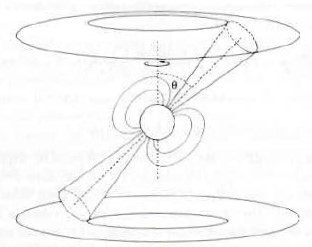
\includegraphics{pulsar.jpg}
    \caption{A pulsar \autocite{maoz}.}
    \label{fig:pulsar1}
\end{figure}

While some pulsars, like the Crab Pulsar \autocite{maoz}, emit electromagnetic waves in the visible spectrum and can therefore be detected by an optical telescope, the majority of pulsar emission is invisible to the human eye and requires a radio telescope to be detected.

\subsubsection{What is a Pulsar Profile?}
\subsubsection{What is multi-path scattering?}
\subsubsection{What is a Pulsar Dispersion Measure?}
\subsubsection{What is a Radio Telescope and how do they work?}
\subsubsection{What is the Murchison Widefield Array?}
\subsubsection{Why are we conducting sky surveys?}
\subsubsection{How is a sky survey conducted with the Murchison Widefield Array?}
\subsubsection{What is tied-array beamforming?}
\subsubsection{How many Pulsar candidates are found in a Murchison Widefield Array sky survey?}
\subsubsection{How long do sky surveys take?}
\subsubsection{How much data is created from a sky survey?}
\subsubsection{What is Radio Frequency Interference?}
\subsubsection{What is a Signal-to-Noise Ratio?}
\subsubsection{What is PRESTO and a .PFD file?}
\subsubsection{What is Machine Learning?}
\subsubsection{How does Machine Learning work?}
\subsubsection{Why do we need to use Machine Learning in finding new Pulsars?}
\subsubsection{Why is this particular Machine Learning Classifier used?}


\pagebreak
% Methods Section
\section{Methods}
\subsection{Developing the Machine Learning Training Dataset}

Before a machine learning algorithm can make predictions and classify candidates as a pulsar or a non-pulsar, it must first build a classification model from a training dataset which contains similar data with known positive and negative classifications \autocite{tan, lyon}. For the use case of pulsar classification, the training dataset must contain examples of data from both pulsars and from non-pulsars so that the algorithm can learn how to distinguish between the two classes.

To maximise the accuracy of the machine learning algorithm, the input data (including the training dataset) must be composed of a common group of features that can be determined for each candidate that maximises the differences between a pulsar and a non-pulsar. The candidate features used by \smartcite{tan} to maximise the differences between pulsar and non-pulsar candidates are:

\begin{equation}
    Prof_{\mu}, Prof_{\sigma}, Prof_{S}, Prof_{k}
\end{equation}

\begin{equation}
    DM_{\mu}, DM_{\sigma}, DM_{S},DM_{k},
    DM_{\mu'}, DM_{\sigma'}, DM_{|S'|},DM_{k'}
\end{equation}

\begin{equation}
    Subband_{\mu}, Subband_{\sigma}, Subband_{S}, Subband_{k}
\end{equation}

\begin{equation}
    Subint_{\mu}, Subint_{\sigma}, Subint_{S}, Subint_{k}
\end{equation}

Where candidate features are calculated from the: (1) Integrated Pulsar Profile, (2) the Dispersion Measure -- Signal-to-Noise Ratio Curve (DM-S/N), (3) the correlation coefficients between each sub-band and the integrated pulsar profile, and from the (4) correlation coefficients between each sub-integration and the integrated pulsar profile. See \emph{Appendix 2A} for formulae to calculate each feature.

To extract the 20 above features from each classification candidate, we can use the software 
\verb|PulsarFeatureLab| \autocite{lyon}.

\subsubsection{Pulsar Candidate Feature Extraction}

The Python software tool \verb|PulsarFeatureLab| can be used to consume pulsar candidate files of the PRESTO Prepfold \verb|PFD| filetype and output the 20 above features for each candidate into a single file of WEKA Data Mining \verb|ARFF| filetype \autocite{lyon}.

To create a closed software environment in which the dependencies of the \verb|PulsarFeatureLab| software are unaffected by the host operating system, a containerised virtual operating system can be created using the free software Docker (\verb|https://docker.com|).

First, a directory to store the Dockerfile and pulsar candidate data is created by completing the following commands in a UNIX terminal:

\begin{lstlisting}[numbers=none]
$ mkdir ~/pulsars
$ cd ~/pulsars
$ touch Dockerfile
\end{lstlisting}

To create the Docker image, the contents of the \verb|Dockerfile| can be edited to contain:

\begin{lstlisting}[title=Dockerfile]
FROM alpine/git:latest as builder
WORKDIR /root/
RUN cd /root/ && git clone --single-branch --branch V1.3.2 https://github.com/scienceguyrob/PulsarFeatureLab.git && mkdir PulsarFeatureLab/PulsarFeatureLab/Data/IO

FROM python:2.7
WORKDIR /usr/src/app
COPY --from=builder /root/PulsarFeatureLab .
RUN pip install numpy scipy matplotlib astropy
ENTRYPOINT ["python", "./PulsarFeatureLab/Src/PulsarFeatureLab.py"]
\end{lstlisting}

The above \verb|Dockerfile| instructs Docker to:
\begin{enumerate}[label=\roman*.]
    \item use an image of Alpine Linux with \verb|git| preinstalled to download the \verb|PulsarFeatureLab| software from GitHub \\(\verb|https://github.com/scienceguyrob/PulsarFeatureLab|);
    \item create a directory inside the downloaded software to store the input and output data;
    \item create a Docker image based on Python 2.7;
    \item transfer the \verb|PulsarFeatureLab| software into the Python 2.7 image; and
    \item install \verb|PulsarFeatureLab|'s library dependencies (\verb|NumPy, SciPy, matplotlib| and \verb|astropy|).
\end{enumerate}

The above Docker image can now be built into a container (a virtual operating system) and a directory to hold the input data can be created by running the following commands on a UNIX terminal:

\begin{lstlisting}[numbers=none]
$ docker build -t jacobianm/pulsarfeaturelab:1.3.2 .
$ mkdir ~/pulsars/data/pfd
\end{lstlisting}

Candidate \verb|PFD| files of known pulsars and non-pulsars detected by the Murchison Widefield Array (MWA) provided by N. Swainston can now populate the above created directory, and the following command can be ran to extract the features from the candidates:

\begin{lstlisting}[numbers=none]
$ docker run --rm -v ~/pulsars/data/pfd:/usr/src/app/PulsarFeatureLab/Data/IO jacobianm/pulsarfeaturelab:1.3.2 -d "/usr/src/app/PulsarFeatureLab/Data/IO" -c 3 -t 6 -f "/usr/src/app/PulsarFeatureLab/Data/IO/output.arff" --arff --meta
\end{lstlisting}

This function instructs Docker to connect the directory containing the \verb|PFD| files to the \verb|PulsarFeatureLab| container's input/output directory and then run the \verb|PulsarFeatureLab| software with arguments stating where the input files are, what filetype they are (\verb|PFD|), which set of features to extract, and where to place the output file.

\subsubsection{Creating the Training Dataset}

The \verb|output.arff| file created by \verb|PulsarFeatureLab|, contains a set of comma-separated features for each candidate, with an appended `?' character, per file line. Since the class of each candidate is already known, the `?' character on each line can be replaced by a `1' if the candidate is a pulsar, or a `0' if the candidate is a non-pulsar. This signals to the Machine Learning algorithm what a pulsar and a non-pulsar candidate's feature set may appear like.

The edited file can now be renamed and moved with the following command:

\begin{lstlisting}[numbers=none]
$ mv ~/pulsars/data/pfd/output.arff ~/pulsars/data/trainingSet.arff
\end{lstlisting}

The Machine Learning Training Dataset has now been created using Murchison Widefield Array data.
    
\subsection{Evaluating the LOTAASClassifier Machine Learning Classification Tool for use with the Murchison Widefield Array}

To address the Candidate Selection Problem discussed in \emph{Section 1.3} of this report, a Java Machine Learning pulsar classification tool named \verb|LOTAASClassifier| was created to classify the pulsar candidates produced by the LOFAR Tied-Array All-sky Survey (LOTAAS) \autocite{lyon}. Due to the similarities between the LOFAR radio telescope and the Murchison Widefield Array (MWA) radio telescope, it is logical to attempt to apply the \verb|LOTAASClassifier| tool to candidates produced by the MWA.

The \verb|LOTAASClassifier| tool contains four machine learning algorithms with which the user can choose to make pulsar classifications. They are: the J48 (C4.5 Decision Tree \autocite{quinlan}), the Multi-Layer Perceptron, the Naive Bayes, and the Support Vector Machines (SVM) algorithms \autocite{lyon}.

To begin evaluating the software, \verb|LOTAASClassifier v1.0| can be downloaded from its GitHub repository \\(\verb|https://github.com/scienceguyrob/LOTAASClassifier|) with the following UNIX terminal commands:

\begin{lstlisting}[numbers=none]
$ cd ~/pulsars
$ git clone https://github.com/scienceguyrob/LOTAASClassifier.git
\end{lstlisting}

The tool's executable program can then be found by navigating to the following directory in the UNIX terminal:

\begin{lstlisting}[numbers=none]
$ cd ~/pulsars/LOTAASClassifier/dist
\end{lstlisting}

\subsubsection{Creating a Pulsar Classifier Output Validation Tool}

In order to accurately evaluate and test the predictions made by the \verb|LOTAASClassifier| tool, we must create a program that will automate the process of checking the outputs of the classifier against the known list of pulsars.

We begin by creating a new Java project using the free software Maven (\verb|https://maven.apache.org|) by running the following commands in a UNIX terminal:

\begin{lstlisting}[numbers=none]
$ cd ~/pulsars
$ mkdir PulsarValidator && cd PulsarValidator
$ mvn archetype:generate -DarchetypeGroupId=org.apache.maven.archetypes -DarchetypeArtifactId=maven-archetype-quickstart -DarchetypeVersion=1.4
\end{lstlisting}

We can then create the following file structure and resynchronise the project:

\begin{lstlisting}[numbers=none]
PulsarValidator/
    src/
        main/
            java/
                com/jacobianmatthews/pulsarvalidator/
                    PulsarValidator.java
        test/
            ...
    target/
            ...
    pom.xml
\end{lstlisting}

The file: \verb|PulsarValidator.java| stands as the entry-point to the software and will be compiled into an executable \verb|JAR| file upon completion of creating the software.

This software will consume a user inputted \verb|String| containing the path to a file with the list of pulsars included in the dataset classified by the machine learning classifier, a user inputted \verb|String| containing the path to the \verb|.positive| file created by the classifier, and a user inputted \verb|String| containing the path to the \verb|.negative| file created by the classifier\footnote{The '.positive' file contains the candidates classified as pulsars, and the '.negative' file contains the candidates classified as non-pulsars.}. These will be inputted as command-line arguments when the user runs the Java executable file.

To access the user inputted arguments, we can include the following function in the \verb|main(String[] args)| method of the \verb|PulsarValidator.java| class:

\begin{algorithm}[H]
    \caption{getCliVariables(args) (pseudocode)}
    \begin{algorithmic}
        \For{Integer $i=0\rightarrow$ number of arguments in $args$}
            \If{$i$th argument in $args$ is "-v"}
                \State Let Boolean $ValidationMode$ = true
                \State Let String $pulsarListPath$ = ($i+1$)th argument in $args$
                \State Let String $classifierPositive$ = ($i+2$)th argument in $args$
                \State Let String $classifierNegative$ = ($i+3$)th argument in $args$
            \EndIf
        \EndFor
    \end{algorithmic}
\end{algorithm}

We can then use a simple conditional statement after this function is ran to check if the \verb|Boolean ValidationMode| has been set to \verb|true|, to determine whether to continue the validation. The complete Java class \verb|PulsarValidator.java| can be seen in \emph{Appendix 7.2.1}.

We can then create a new Java class, \verb|ValidationMode.java|, with the following algorithm to validate the output of the classifier against the list of pulsars:

\begin{algorithm}[H]
    \caption{ValidationMode.java (pseudocode)}
    \begin{algorithmic}
        \State Let $truePositive$ = new List
        \State Let $falsePositive$ = new List
        \State Let $trueNegative$ = new List
        \State Let $falseNegative$ = new List
        
        \For{each $item$ in $classifierPositive$ list}
            \State Let Boolean $found$ = false
            \State Let Integer $i=0$
            \While{$found$ is false}
                \If{$i$th item in $pulsarList$ is $item$}
                    \State add $item$ to $truePositive$ list
                    \State $found$ = true
                \ElsIf{$i$ equals number of items in $pulsarList$}
                    \State add $item$ to $falsePositive$ list
                    \State $found$ = true
                \Else
                    \State $i$=$i+1$
                \EndIf
            \EndWhile
        \EndFor

        \For{each $item$ in $classifierNegative$ list}
            \State Let Boolean $found$ = false
            \State Let Integer $i=0$
            \While{$found$ is false}
                \If{$i$th item in $pulsarList$ is $item$}
                    \State add $item$ to $falseNegative$ list
                    \State $found$ = true
                \ElsIf{$i$ equals number of items in $pulsarList$}
                    \State add $item$ to $truePositive$ list
                    \State $found$ = true
                \Else
                    \State $i$=$i+1$
                \EndIf
            \EndWhile
        \EndFor
        \State Let $TP$ = number of items in $truePositive$
        \State Let $TN$ = number of items in $trueNegative$
        \State Let $FP$ = number of items in $falsePositive$
        \State Let $FN$ = number of items in $falseNegative$
        \State Let $Pulsars$ = $TP+FN$
        \State Let $NonPulsars$ = $TN+FP$
        \State Output $Pulsars$, $NonPulsars$, $TP$, $FP$, $TN$, $FN$
    \end{algorithmic}
\end{algorithm}

The complete Java class for \verb|ValidationMode.java| can be found in \emph{Appendix 7.2.2}, and its supplementary classes in \emph{Appendix 7.2}.

We can now compile the program by first adding the following lines of code to the \verb|pom.xml| file at the root of the Maven project:

\begin{lstlisting}[numbers=none, title=pom.xml]
<project>
  ...
  <build>
    ...
    <pluginManagement>
      ...
      <plugins>
        ...
        <!-- Create a JAR containing the resources and dependencies -->
        <plugin>
          <artifactId>maven-assembly-plugin</artifactId>
          <configuration>
            <descriptorRefs>
              <descriptorRef>jar-with-dependencies</descriptorRef>
            </descriptorRefs>
            <finalName>${project.artifactId}-${project.version}-full</finalName>
            <appendAssemblyId>false</appendAssemblyId>
            <archive>
              <manifest>
                <mainClass>com.jacobianmatthews.pulsarvalidator.PulsarValidator</mainClass>
              </manifest>
            </archive>
          </configuration>
          <executions>
            <execution>
                <id>make-my-jar-with-dependenciess</id>
                <phase>package</phase>
                <goals>
                    <goal>single</goal>
                </goals>
            </execution>
          </executions>
        </plugin>
      </plugins>
    </pluginManagement>
  </build>
</project>
\end{lstlisting}

Which instructs Maven to create a single \verb|JAR| file containing the program's dependencies and resources. The program can then be compiled and built by running the command:

\begin{lstlisting}[numbers=none]
$ mvn assembly:single
\end{lstlisting}

This will produce the file: \verb|/target/pulsarvalidator-1.0-full.jar|, which is an executable Java program. The complete source code for \verb|PulsarValidator| can be found in \emph{Appendix 7.2} or at \\\verb|https://github.com/jacob-ian/PulsarValidator.git|.

\subsubsection{Creating a Classification Model}

In order to use \verb|LOTAASClassifier| to classify Murchison Widefield Array candidates, we must use the Machine Learning Training Dataset created in \emph{Section 2.1} to create a classification model. This can be completed by running the following commands:

\begin{lstlisting}[numbers=none]
$ java -jar LOTAASClassifier.jar -t ~/pulsars/data/trainingSet.arff -m ~/pulsars/data/model.m -a 1
\end{lstlisting}

This instructs \verb|LOTAASClassifier| to create a new classification model for the J48 machine learning algorithm with the previously constructed training dataset.

To ensure that the classification model was created successfully, we can test the model against the same dataset provided by N. Swainston to create the training dataset. Using \verb|PulsarFeatureLab| we can produce a new \verb|output.arff| file with the candidates' class unedited.

\begin{lstlisting}[numbers=none]
$ docker run --rm -v ~/pulsars/data/pfd:/usr/src/app/PulsarFeatureLab/Data/IO jacobianm/pulsarfeaturelab:1.3.2 -d "/usr/src/app/PulsarFeatureLab/Data/IO" -c 3 -t 6 -f "/usr/src/app/PulsarFeatureLab/Data/IO/output.arff" --arff --meta
\end{lstlisting}

It is now possible to test the classification model with the candidate feature sets with the following commands:

\begin{lstlisting}[numbers=none]
$ cd ~/pulsars/LOTAASClassifier/dist
$ java -jar LOTAASClassifier.jar -p ~/pulsars/data/pfd/output.arff -m ~/pulsars/data/model.m -a 1
\end{lstlisting}

The \verb|LOTAASClassifier| tool will output two files: `\verb|output.positive|' and `\verb|output.negative|', in the same location as the input dataset. The J48 classification model was constructed successfully if the candidates inside the `\verb|positive|' file are the known pulsars.

\subsubsection{Evaluating LOTAASClassifier}

With a successfully created machine learning classification model, it is now possible to test \verb|LOTAASClassifier| against a previously unseen (by the classifier) dataset of Murchison Widefield Array candidates whose class is also known. We can first remove the existing candidates from inside the \verb|PFD| files directory and delete the existing \verb|output| files.

The candidates directory can then be populated by new \verb|PFD| files and we can use the `\verb|docker run|' command from \emph{Section 2.2.1} to extract the features from the new candidates.

The \verb|LOTAASClassifier| tool can now make classification predictions on the new candidates by running the UNIX terminal command:

\begin{lstlisting}[numbers=none]
$ cd ~/pulsars/LOTAASClassifier/dist
$ java -jar LOTAASClassifier.jar -p ~/pulsars/data/pfd/output.arff -m ~/pulsars/data/model.m -a 1
\end{lstlisting}

This can be repeated for each machine learning classifier present in the \verb|LOTAASClassifier| software by changing the argument \verb|-a| from 1 through to 4.

We can now run the \verb|PulsarValidator| program created in \emph{Section 2.2.1} to evaluate the accuracy of \verb|LOTAASClassifier|'s algorithms by running the command:

\begin{lstlisting}[numbers=none]
$ cd ~/pulsars/PulsarValidator/target
$ java -jar pulsarvalidator-1.0-full.jar -v ~/pulsars/data/pfd/pulsars.txt ~/pulsars/data/pfd/output_[classifier].positive ~/pulsars/data/pfd/output_[classifier].negative
\end{lstlisting}

Where the \verb|[classifier]| variable can be changed depending on the name of the classifier algorithm being evaluated. The outputted validation statistics can then be compared across the algorithms to determine their usefulness with the Murchison Widefield Array.

\subsubsection{Creating the PulsarClassifier Ensemble Classification Tool}

According to \cite{tan}, using Machine Learning algorithms in ensemble to make pulsar classifications increases the accuracy of classifications, classifying pulsars that were often misclassified such as wide-pulse pulsars.

To build the ensemble classification feature into the existing \verb|LOTAASClassifier| tool, we can first begin by creating a new Java project named \verb|PulsarClassifier| using the free software, Maven (\verb|https://maven.apache.org|).

\begin{lstlisting}[numbers=none]
$ cd ~/pulsars
$ mkdir PulsarClassifier && cd PulsarClassifier
$ mvn archetype:generate -DarchetypeGroupId=org.apache.maven.archetypes -DarchetypeArtifactId=maven-archetype-quickstart -DarchetypeVersion=1.4
\end{lstlisting}

We can now copy the source code from \verb|LOTAASClassifier| to be included in the \verb|PulsarClassifier| software.

\begin{lstlisting}[numbers=none]
$ cp -R ~/pulsars/LOTAASClassifier/src/ ~/pulsars/PulsarClassifier/src/main/java
\end{lstlisting}

To use the WEKA suite of Machine Learning tools, we must then edit the \verb|pom.xml| file inside \verb|PulsarClassifier| to include it as a dependency, and resynchronise the project:\\

\begin{lstlisting}[numbers=none, title=pom.xml, language=xml]
...
<dependencies>
...
    <dependency>
        <groupId>nz.ac.waikato.cms.weka</groupId>
        <artifactId>weka-stable</artifactId>
        <version>3.8.0</version>
    </dependency>
...
</dependencies>
...
\end{lstlisting}

We now have the following basic project directory structure:

\begin{lstlisting}[numbers=none]
PulsarClassifier/
    src/
        main/
            java/
                com/jacobianmatthews/pulsarclassifier/
                com/scienceguyrob/lotaasclassifier/
        test/
            java/
                com/jacobianmatthews/pulsarclassifier
    target/
            ...
    pom.xml
\end{lstlisting}

Where the new source code will be located under \\\verb|/src/main/java/com/jacobianmatthews/pulsarclassifier|. To introduce the ensemble classification feature, we must write four main Java classes: \\\verb|PulsarClassifier.java|,  \verb|ClassifierBuilder.java|,  \verb|ClassifierValidator.java|,  and \verb|ClassPredictor.java|.

The \verb|LOTAASClassifier| tool accepts a command-line argument \verb|-a| which accepts an integer that denotes the machine learning algorithm to use in building a classification model and making predictions \autocite{lyon}. Therefore, we will add an algorithm into the above listed Java classes that will accept an integer value of \verb|-1| that will activate the ensemble classifier.

The class \verb|ClassifierBuilder.java| handles training and building a classification model. To add ensemble classification to this class we will use the following algorithm:

\begin{algorithm}[H]
    \caption{ClassifierBuilder (pseudocode)}
    \begin{algorithmic}[1]
        \If{$algorithm = -1$}
            \For{each algorithm $i=1\rightarrow 4$}
                \Comment Loop through all classifiers
                \State buildClassifier($i$, $trainingSet$, $modelsDirectory$)
            \EndFor
        \Else 
            \Comment Build individual classifier
            \State buildClassifier($algorithm$, $trainingSet$, $modelPath$)
            
        \EndIf
        
    \end{algorithmic}
\end{algorithm}

\emph{See Section 8.4.1} for complete \verb|ClassifierBuilder.java| class. 

The class \verb|ClassifierValidator.java| handles validating and testing the existing classification models. To implement the ensemble classifier into this class, we will use the following, similar algorithm:

\begin{algorithm}[H]
    \caption{ClassifierValidator (pseudocode)}
    \begin{algorithmic}[1]
        \If{$algorithm = -1$}
            \For{each algorithm $i=1\rightarrow 4$}
                \Comment Loop through all classifiers
                \State testClassifier($i$, $testSet$, $modelsDirectory$)
            \EndFor
        \Else 
            \Comment Test individual classifier
            \State testClassifier($algorithm$, $testSet$, $modelPath$)
        \EndIf
        
    \end{algorithmic}
\end{algorithm}

\emph{See Section 8.4.2} for complete \verb|ClassifierValidator.java| class. 

The class \verb|ClassPredictor.java| handles making the classification predictions on new data using existing classifier models. We can add the ensemble classification feature to this class with the following algorithm:

\begin{algorithm}[H]
    \caption{ClassPredictor (pseudocode)}
    \begin{algorithmic}[1]
        \If{$algorithm = -1$}
            \State list = new OutputFileList()
            \For{algorithm $i=1\rightarrow4$}
                \Comment Loop through all classifiers
                \State makePredictions($i$, $inputData$, $modelsDirectory$)
                \State list.add(ClassifierOutputFiles)
                \Comment Add output filepaths to list
            \EndFor
            \State positiveList = new ClassificationsList()
            \State negativeList = new ClassificationsList()
            \Comment Create classification lists
            \For{each OutputFile from list}
                \If{OutputFile is .positive}
                    \For{each line in OutputFile}
                        \State positiveList.add(line)
                        \Comment Add to +ve classifications
                    \EndFor
                \ElsIf{OutputFile is .negative}
                    \For{each line in OutputFile}
                        \State negativeList.add(line)
                        \Comment Add to -ve classifications
                    \EndFor
                \EndIf
            \EndFor
            \For{each classification in positiveList}
                \If{classification.occurrences $< 3$}
                    \State negativeList.add(classification)
                    \Comment cut-off at $< 3$ classifications
                \Else
                    \State positiveOutput(classification)
                    \Comment Output classified as Pulsar
                \EndIf
            \EndFor
            \For{each classification in negativeList}
                \State negativeOutput(classification)
                \Comment Output classified as non-Pulsar
            \EndFor

        \Else 
            \State makePredictions($algorithm$)
            \Comment Use individual classifier
        \EndIf
        
    \end{algorithmic}
\end{algorithm}

The above algorithm preserves the individual classifiers' predictions and also makes an ensemble prediction based on all of the classifiers' predictions. According to \cite{tan}, it is common for ensemble machine learning classifiers to use a cut-off of three concurrent positive predictions in separate classifiers to make a positive ensemble classification. Therefore, for a candidate to be classified as a pulsar with the ensemble classifier it must first be classified as a pulsar by three of the underlying machine learning classifiers. \emph{See Section 8.4.3} for the complete \verb|ClassPredictor.java| class.

The final class to add the ensemble classifier feature to is the entry point of the program, \verb|PulsarClassifier.java|. This class only requires changes to the command-line inputs and outputs, so the completed Java class can be found in \emph{Section 8.4.4}. The complete source code to the \verb|PulsarClassifier| contains the following classes:

\begin{lstlisting}[numbers=none]
src/
    main/
        java/
            com/jacobianmatthews/pulsarclassifier/
                utils/
                    Classification.java
                    ClassificationList.java
                    Classifiers.java
                    Models.java
                PulsarClassifier.java
                ClassifierBuilder.java
                ClassifierValidator.java
                ClassPredictor.java

            com/scienceguyrob/lotaasclassifier/
                ...

\end{lstlisting}

Now that the source code for the package is complete, we can add the following lines to the \verb|pom.xml| file at the root of the project:

\pagebreak
\begin{lstlisting}[numbers=none, language=xml, title=pom.xml, basicstyle=\footnotesize\ttfamily]
<project>
    ...
    <build>
      <pluginManagement>
        <plugins>
          ...

          <!-- Create a JAR containing the resources and dependencies -->
          <plugin>
            <groupId>org.apache.maven.plugins</groupId>
            <artifactId>maven-assembly-plugin</artifactId>
            <configuration>
              <archive>
                <manifest>
                  <addClasspath>true</addClasspath>
                  <mainClass>com.jacobianmatthews.pulsarclassifier.PulsarClassifier</mainClass>
                </manifest>
              </archive>
              <descriptorRefs>
                <descriptorRef>jar-with-dependencies</descriptorRef>
              </descriptorRefs>
            </configuration>
            <executions>
              <execution>
                <phase>package</phase>
                <goals>
                  <goal>single</goal>
                </goals>
              </execution>
            </executions>
          </plugin>

          ...
        </plugins>
      </pluginManagement>
    </build>
    ...
</project>
\end{lstlisting}

This will instruct Maven to build a Java \verb|JAR| file containing the package and its WEKA library dependency. To build the package, we can run the following commands in the UNIX terminal:

\begin{lstlisting}[numbers=none]
$ cd ~/pulsars/PulsarClassifier
$ mvn assembly:single
\end{lstlisting}

The complete source code and build of \verb|PulsarClassifier| can be found at \verb|https://github.com/jacob-ian/PulsarClassifier.git|, or in \emph{Appendix 7.3}.

\subsubsection{Evaluating PulsarClassifier}

Now that we have successfully built \verb|PulsarClassifier|, we can evaluate its usage with the Murchison Widefield Array's (MWA) candidates. We begin by:
\begin{enumerate}[label=\roman*.] 
    \item deleting the previous \verb|output.positive| and \verb|output.negative| files from the \verb|PFD| candidates directory; and
    \item deleting the previous \verb|model.m| file created by the \verb|LOTAASClassifier| software.
\end{enumerate}

We can now build the ensemble classification model with the training dataset created earlier, by running the following commands:

\begin{lstlisting}[numbers=none]
$ cd target
$ java -jar pulsarclassifier-1.0-jar-with-dependencies.jar -t ~/pulsars/data/trainingSet.arff -m ~/pulsars/data/models -a -1
\end{lstlisting}

Where the argument \verb|-m| now denotes the path to a directory to store the various classifier models. Now that we have all of the classification models created, we can use the ensemble classifier to predict the class of new candidates. Using the feature extracted candidates compiled from \emph{Section 2.2.2}, we can run the following command:

\begin{lstlisting}[numbers=none]
$ java -jar pulsarclassifier-1.0-jar-with-dependencies.jar -p ~/pulsars/data/pfd/output.arff -m ~/pulsars/data/models -a -1
\end{lstlisting}

\verb|PulsarClassifier| will create the prediction output files for each classifier, and then the \verb|output_ensemble.positive| and \verb|output_ensemble.negative| files for the ensemble classifier. We can validate the ensemble classifier with the \verb|PulsarValidator| program created in \emph{Section 2.2.1} by running the commands:

\begin{lstlisting}[numbers=none]
$ cd ~/pulsars/PulsarValidator/target
$ java -jar pulsarvalidator-1.0-full.jar -v ~/pulsars/data/pfd/pulsars.txt ~/pulsars/data/pfd/output_ensemble.positive ~/pulsars/data/pfd/output_ensemble.negative
\end{lstlisting}

The outputted validation statistics can then be compared to those created for the \verb|LOTAASClassifier| algorithms and an opinion can be formed in regards to the utility of \verb|PulsarClassifier| with the Murchison Widefield Array.

\pagebreak
% Results Section
\section{Results and Analyses}
\subsection{Machine Learning Training Dataset}

The machine learning training dataset created with candidates detected by the Murchison Widefield Array can be found under \emph{Appendix 7.1}.

\subsection{Classification Results from the LOTAASClassifier Algorithms}

\subsubsection{The J48 Algorithm}

The output created by \verb|PulsarValidator| on analysis of the classification results of the J48 (C4.5 Decision Tree) algorithm is as follows:

\begin{lstlisting}[numbers=none]
Number of Pulsars: 147
Pulsars Detected: 146
True Positives: 131
False Positives: 15

Number of Non-Pulsars: 87
Non-Pulsars Detected: 88
True Negatives: 72
False Negatives: 16
\end{lstlisting}

We can therefore calculate the pulsar classification success rate to be:

$$ R_{p} = \frac{TP}{N_p} = \frac{131}{147} =  0.8911 = 89.11\%,$$

where $N_p$ is the number of pulsars in the testing dataset and $TP$ is the number of true positive classifications. The non-pulsar classification success rate can be found as:

$$R_{np} = \frac{TN}{N_{np}} = \frac{72}{87} = 0.8275 = 82.75\%,$$

where $N_{np}$ is the number of non-pulsars in the testing dataset and $TN$ is the number of true negative classifications.

\subsubsection{The Multi-Layer Perceptron Algorithm}

The output created by \verb|PulsarValidator| on analysis of the classification results of the Multi-Layer Perceptron algorithm is as follows:

\begin{lstlisting}[numbers=none]
Number of Pulsars: 147
Pulsars Detected: 125
True Positives: 123
False Positives: 2

Number of Non-Pulsars: 87
Non-Pulsars Detected: 109
True Negatives: 85
False Negatives: 24
\end{lstlisting}

We can therefore calculate the pulsar classification success rate to be:

$$ R_{p} = \frac{TP}{N} = \frac{123}{147} =  0.8367 = 83.67\%,$$

where $N$ is the number of pulsars in the testing dataset, and $TP$ is the number of true positive classifications. The non-pulsar classification success rate can be found as:

$$R_{np} = \frac{TN}{N_{np}} = \frac{85}{87} = 0.9770 = 97.70\%,$$

where $N_{np}$ is the number of non-pulsars in the testing dataset and $TN$ is the number of true negative classifications.

\subsubsection{The Naïve Bayes Tester Algorithm}

The output created by \verb|PulsarValidator| on analysis of the classification results of the Naïve Bayes algorithm is as follows:

\begin{lstlisting}[numbers=none]
Number of Pulsars: 147
Pulsars Detected: 119
True Positives: 118
False Positives: 1

Number of Non-Pulsars: 87
Non-Pulsars Detected: 115
True Negatives: 86
False Negatives: 29
\end{lstlisting}

We can therefore calculate the pulsar classification success rate to be:

$$ R_{p} = \frac{TP}{N} = \frac{118}{147} =  0.8027 = 80.27\%,$$

where $N$ is the number of pulsars in the testing dataset, and $TP$ is the number of true positive classifications. The non-pulsar classification success rate can be found as:

$$R_{np} = \frac{TN}{N_{np}} = \frac{86}{87} = 0.9885 = 98.85\%,$$

where $N_{np}$ is the number of non-pulsars in the testing dataset and $TN$ is the number of true negative classifications.

\subsubsection{The Support Vector Machine Algorithm}

The output created by \verb|PulsarValidator| on analysis of the classification results of the Naïve Bayes algorithm is as follows:

\begin{lstlisting}[numbers=none]
Number of Pulsars: 147
Pulsars Detected: 97
True Positives: 97
False Positives: 0

Number of Non-Pulsars: 87
Non-Pulsars Detected: 137
True Negatives: 87
False Negatives: 50
\end{lstlisting}

We can therefore calculate the pulsar classification success rate to be:

$$ R_{p} = \frac{TP}{N} = \frac{97}{147} =  0.6598 = 65.98\%,$$

where $N$ is the number of pulsars in the testing dataset, and $TP$ is the number of true positive classifications. The non-pulsar classification success rate can be found as:

$$R_{np} = \frac{TN}{N_{np}} = \frac{87}{87} = 1.00 = 100.00\%,$$

where $N_{np}$ is the number of non-pulsars in the testing dataset and $TN$ is the number of true negative classifications.

\subsection{Classification Results from the PulsarClassifier Ensemble Classifier}

The output created by \verb|PulsarValidator| on analysis of the classification results of the \verb|PulsarClassifier| ensemble classifier is as follows:

\begin{lstlisting}[numbers=none]
Number of Pulsars: 147
Pulsars Detected: 112
True Positives: 112
False Positives: 0

Number of Non-Pulsars: 87
Non-Pulsars Detected: 122
True Negatives: 87
False Negatives: 35
\end{lstlisting}

We can therefore calculate the pulsar classification success rate to be:

$$ R_{p} = \frac{TP}{N} = \frac{112}{147} =  0.7619 = 76.19\%,$$

where $N$ is the number of pulsars in the testing dataset, and $TP$ is the number of true positive classifications. The non-pulsar classification success rate can be found as:

$$R_{np} = \frac{TN}{N_{np}} = \frac{87}{87} = 1.00 = 100.00\%,$$

where $N_{np}$ is the number of non-pulsars in the testing dataset and $TN$ is the number of true negative classifications.

\subsection{Combined Analyses}

A table containing the pulsar and non-pulsar classification success rates of all algorithms and the ensemble classifier can be found below:

\begin{table}[H]
    \centering
    
    \caption{Success Rates of Each Pulsar Classifier}

    \begin{framed}
        \begin{tabular}{l c c c}
            Classifier & $R_p$ & $R_{np}$ & $Combined$ \\
            \hline
            \hline
            LOTAASClassifier &  &  & \\
            \hline
            J48 & 89.11\% & 82.75\% & 85.93\% \\
            MLP & 83.67\% & 97.70\% & 90.69\% \\
            NB & 80.27\% & 98.85\% & 89.56\%\\
            SVM & 65.98\% & 100.00\% & 82.99\% \\
            \hline
            PulsarClassifier &  &  & \\
            \hline
            Ensemble & 76.19\% & 100.00\% & 88.10\% \\
        \end{tabular}
    \end{framed}
    \label{tab:analyses}
\end{table}

\pagebreak
% Results Discussion Section
\section{Discussion and Conclusions}
\subsection{How effective is the chosen training dataset?}
\subsection{Evaluating Curtin Institute of Radio Astronomy's Pulsar Classification Pipeline}
\subsection{Why did/didn't the LOFAR Machine Learning Algorithm work with the MWA?}
\subsection{What changes to the algorithm were necessary for it to successfully classify Pulsars from the MWA?}

\pagebreak
% RECOMMENDATIONS SECTION
\section{Recommendations}

For further development of the Machine Learning classifiers and strategies used in this project, I would recommend undertaking the following tasks:

\begin{enumerate}
    \item Investigate and fix the Python \verb|Traceback| Error produced by the software \verb|PulsarFeatureLab v1.3.2|:

    During the usage of this feature extraction software, some \verb|PFD| candidate files would cause a \verb|Traceback| error to be produced, causing the feature extraction to fail for that particular candidate. In the \verb|PFD| datasets that I used, the only commonality between the failed feature extraction candidates was that the candidates were not pulsars - they were either examples of Radio Frequency Interference (RFI) or Noise. The result of these failures was that there was a smaller dataset to train the machine learning classifiers on, or a smaller dataset to make machine learning classification predictions on.

    \item Build the Radio Frequency Interference (RFI) classification feature discussed by \textcite{tan} into \verb|PulsarClassifier|:
    
    According to \textcite{tan}, by also including the classification category of RFI, the accuracy of the machine learning ensemble classifier was increased. The result of this feature would be three classifier output files: \verb|output.pulsars|, \verb|output.rfi|, and \verb|output.other|.

    \item Use a more diverse Training Dataset:

    Due to constraints on the available \verb|PFD| candidate data during this project, I was unable to use a large set of pulsar and non-pulsar candidates in the training dataset. By using a training dataset that is more diverse, the \verb|PulsarClassifier| will be more accurate in its predictions.
\end{enumerate}

\pagebreak
% REFERENCES SECTION
\section{References}
\printbibliography[heading=none]

\pagebreak
% APPENDICES SECTION
\section{Appendices}
\subsection{Machine Learning Training Dataset}
\lstinputlisting[title=trainingData.arff, basicstyle=\footnotesize\ttfamily, breaklines=true, framexleftmargin=2.5em]{code/trainingSet.arff}

\pagebreak
\subsection{PulsarValidator}
\subsubsection{PulsarValidator.java}
\lstinputlisting[title=PulsarValidator.java, language=Java, basicstyle=\footnotesize\ttfamily, breaklines=true, framexleftmargin=2.5em]{code/jacobianmatthews/pulsarvalidator/PulsarValidator.java}

\pagebreak
\subsubsection{ValidationMode.java}
\lstinputlisting[title=ValidationMode.java, language=Java, basicstyle=\footnotesize\ttfamily, breaklines=true, framexleftmargin=2.5em]{code/jacobianmatthews/pulsarvalidator/ValidationMode.java}

\pagebreak
\subsubsection{utils/Statistic.java}
\lstinputlisting[title=utils/Statistic.java, language=Java, basicstyle=\footnotesize\ttfamily, breaklines=true, framexleftmargin=2.5em]{code/jacobianmatthews/pulsarvalidator/utils/Statistic.java}

\pagebreak
\subsubsection{utils/StatisticList.java}
\lstinputlisting[title=utils/StatisticList.java, language=Java, basicstyle=\footnotesize\ttfamily, breaklines=true, framexleftmargin=2.5em]{code/jacobianmatthews/pulsarvalidator/utils/StatisticList.java}

\pagebreak
\subsubsection{utils/Utilities.java}
\lstinputlisting[title=utils/Utilities.java, language=Java, basicstyle=\footnotesize\ttfamily, breaklines=true, framexleftmargin=2.5em]{code/jacobianmatthews/pulsarvalidator/utils/Utilities.java}

\pagebreak
\subsection{PulsarClassifier}

\subsubsection{PulsarClasifier.java}
\lstinputlisting[title=PulsarClassifier.java, language=Java, basicstyle=\footnotesize\ttfamily, breaklines=true, framexleftmargin=2.5em]{code/jacobianmatthews/pulsarclassifier/PulsarClassifier.java}

\pagebreak
\subsubsection{ClassifierBuilder.java}
\lstinputlisting[title=ClassifierBuilder.java, language=Java, basicstyle=\footnotesize\ttfamily, breaklines=true, framexleftmargin=2.5em]{code/jacobianmatthews/pulsarclassifier/ClassifierBuilder.java}

\pagebreak
\subsubsection{ClassifierValidator.java}
\lstinputlisting[title=ClassifierValidator.java, language=Java, basicstyle=\footnotesize\ttfamily, breaklines=true, framexleftmargin=2.5em]{code/jacobianmatthews/pulsarclassifier/ClassifierValidator.java}

\pagebreak
\subsubsection{ClassPredictor.java}
\lstinputlisting[title=ClassPredictor.java, language=Java, basicstyle=\footnotesize\ttfamily, breaklines=true, framexleftmargin=2.5em]{code/jacobianmatthews/pulsarclassifier/ClassPredictor.java}

\pagebreak
\subsubsection{utils/Classification.java}
\lstinputlisting[title=utils/Classification.java, language=Java, basicstyle=\footnotesize\ttfamily, breaklines=true,framexleftmargin=2.5em]{code/jacobianmatthews/pulsarclassifier/utils/Classification.java}

\pagebreak
\subsubsection{utils/ClassificationList.java}
\lstinputlisting[title=utils/ClassificationList.java, language=Java, basicstyle=\footnotesize\ttfamily, breaklines=true,framexleftmargin=2.5em]{code/jacobianmatthews/pulsarclassifier/utils/ClassificationList.java}

\pagebreak
\subsubsection{utils/Classifiers.java}
\lstinputlisting[title=utils/Classifiers.java, language=Java, basicstyle=\footnotesize\ttfamily, breaklines=true, framexleftmargin=2.5em]{code/jacobianmatthews/pulsarclassifier/utils/Classifiers.java}

\pagebreak
\subsubsection{utils/Models.java}
\lstinputlisting[title=utils/Models.java, language=Java, basicstyle=\footnotesize\ttfamily, breaklines=true, framexleftmargin=2.5em]{code/jacobianmatthews/pulsarclassifier/utils/Models.java}


% End the document
\end{document}